\documentclass[11pt,a4paper]{article}
\usepackage[T1]{fontenc}
\usepackage[utf8]{inputenc}
\usepackage{mathptmx}
\usepackage{helvet,courier}
\usepackage[margin=24mm,headheight=15pt]{geometry}
\usepackage{amsmath,amssymb,graphicx,booktabs,array,longtable}
\usepackage[table]{xcolor}
\usepackage{microtype}
\usepackage{caption}
\usepackage{fancyhdr}
\usepackage[numbers,sort&compress]{natbib}
\ifdefined\submissionformat
\usepackage{setspace}
\usepackage{lineno}
\doublespacing
\AtBeginDocument{\linenumbers}
\fi
\usepackage{hyperref}
\input{glyphtounicode}
\pdfgentounicode=1
\definecolor{navy}{HTML}{183B56}
\definecolor{teal}{HTML}{167D8D}
\hypersetup{colorlinks=true,linkcolor=navy,citecolor=navy,urlcolor=teal,pdfauthor={},pdftitle={Graph-based exploration of chemical-disease associations}}
\captionsetup{font=small,labelfont=bf,labelsep=period}
\setlength{\parskip}{4pt}
\setlength{\parindent}{1em}
\setlength{\emergencystretch}{2em}
\renewcommand{\topfraction}{0.95}
\renewcommand{\bottomfraction}{0.9}
\renewcommand{\textfraction}{0.05}
\renewcommand{\floatpagefraction}{0.85}
\setcounter{topnumber}{3}
\setcounter{totalnumber}{5}
\renewcommand{\arraystretch}{1.18}
\pagestyle{fancy}
\fancyhf{}
\fancyhead[L]{\small\sffamily Chemical-disease association analysis}
\fancyhead[R]{\small\sffamily Draft for author review}
\fancyfoot[C]{\small\thepage}
\renewcommand{\headrulewidth}{0.3pt}
\newcommand{\blankfield}[1]{\noindent\textbf{#1}\ \rule{0.68\linewidth}{0.3pt}\par}
\newcommand{\sourceitem}[1]{\textsf{#1}}
\graphicspath{{../figures/}}

\begin{document}
\ifdefined\submissionformat\thispagestyle{plain}\else\thispagestyle{empty}\fi
\begin{center}
{\small\sffamily\color{teal} RESEARCH ARTICLE \quad | \quad EXPLORATORY STUDY}\par
\vspace{8pt}
{\LARGE\bfseries Graph-based exploration of chemical--disease associations with literature and gene-context evidence\par}
\vspace{14pt}
\end{center}
\blankfield{Authors:}
\blankfield{Affiliations:}
\blankfield{Correspondence:}
\vspace{6pt}
\begin{abstract}
\noindent\textbf{Background:} Chemical--disease databases combine environmental exposures, therapeutic effects and inferred associations. Graph learning can prioritize relationships for review, but prediction scores, retrievable publications and shared genes represent different forms of evidence. We examine how these layers can support an evidence-linked chemical--disease workflow.

\noindent\textbf{Methods:} We combined a retrospective assessment of existing graph-learning experiments with descriptive analysis of retained prediction records, aggregate literature-retrieval results and a shared-gene screen. The study inventory reports 9,546,982 Comparative Toxicogenomics Database (CTD) relationship records and 3,125 manually extracted exposure records. The retained code defines a two-layer GraphSAGE baseline for the chemical--disease modeling component; literature and gene overlap provide separate evidence views.

\noindent\textbf{Results:} In the reported exposure-data pilot, a multilayer perceptron achieved an area under the receiver operating characteristic curve of 0.9392, compared with 0.9382 for a graph attention network and 0.9254 for a graph convolutional network. Reported literature-retrieval yield was 30.4\% in the highest-ranked 1,000-record sample and 7.2\% in 1,000 random pairs, a descriptive ratio of 4.22. The retained ranking contains 62,042 misclassified records and lacks class labels; its scores cannot be interpreted uniformly as association probabilities. A separate shared-gene screen reported 128 supported records among 639 mappable records in a 1,000-record sample. The overall rate, 12.8\%, was below the recorded disease-label permutation mean of 18.7\%.

\noindent\textbf{Conclusions:} The results motivate literature-guided review of chemical--disease predictions but do not establish prospective discovery, causal effects or superiority of graph learning. An extensible evidence interface should preserve relation type, denominator, source publication and gene-path provenance. Broader chemical coverage and closer Acemap integration are specified as extensions, with validation requiring reproducible predictions and independent evidence.
\end{abstract}
\noindent\textbf{Keywords:} chemical--disease associations; comparative toxicogenomics; graph neural networks; literature evidence; environmental exposure; knowledge graphs

\section{Background}
Environmental and pharmacological chemicals interact with biological systems across a wide range of exposure settings. Their recorded relationships with disease can describe adverse effects, treatment, molecular perturbation or statistical association. These meanings matter when a database is used to generate hypotheses: a chemical that treats a condition and a chemical associated with increased risk should not become indistinguishable evidence merely because both connect to the same disease node.

The Comparative Toxicogenomics Database (CTD) organizes literature-curated chemical, gene and disease knowledge and derives additional relationships through shared biological information \citep{ctd2025}. It offers an appropriate foundation for broad chemical--disease analysis, while manually extracted environmental studies can add exposure concentration, population and effect-estimate context. These resources differ in their units of evidence. A curated record, an inferred relationship and an epidemiological observation are not interchangeable measurements, and several records may refer to the same chemical--disease pair.

Graph learning provides a way to use the organization of observed relationships when scoring candidate pairs. Graph convolutional networks (GCNs), graph attention networks (GATs) and GraphSAGE aggregate information over neighborhoods using different operators \citep{gcn,gat,graphsage}. In drug--disease prediction, layer-attention GCNs incorporate similarity networks and combine information across layers, while multi-relational approaches integrate additional biological relations \citep{lagcn,mrdda}. These methods motivate graph-based exploration, but their published performance does not establish performance on a different chemical inventory or evaluation split.

For a scientific discovery interface, a score becomes more useful when the user can examine the evidence behind a candidate. Three questions are distinct: whether a model ranks a recorded relationship highly, whether a publication discusses the pair, and whether a biological path provides relevant mechanistic context. Literature retrieval can recover a treatment report or an indirect adverse-event pathway; shared genes can arise because certain genes and diseases are extensively studied. Neither signal alone establishes a new causal relationship.

This study organizes an existing chemical--disease project around these distinctions. We describe the implemented association-modeling baseline, examine the available pilot and evidence-review results, and formulate an evidence-linked interface for broader chemical coverage. The contribution is an exploratory workflow and a quantitative account of its evidence limits, rather than a new graph architecture. We ask whether the reported rankings yield useful literature leads, whether simple gene overlap strengthens their interpretation, and what information must be preserved before candidate relationships can be presented as discoveries.

\section{Methods}
\subsection{Study design and evidence sources}
The analysis has three components: a pilot comparison on literature-extracted exposure data, retrospective examination of CTD-based prediction records, and separate literature and gene-context screens. The database inventory and original pilot metrics are study-level summaries. We additionally counted and characterized the retained prediction CSV directly. Source-level provenance and the distinction between reported and recomputed quantities are provided in Supplementary Information, Tables S1--S4.

The study inventory comprises 9,546,982 CTD chemical--disease relationship records and 3,125 environmental exposure records extracted manually from epidemiological literature (Table~\ref{tab:data}). The inventory reports 108,217 CTD records with direct evidence. These are historical project counts; they do not describe the size of the current CTD release. A relationship record may encode an evidence type or an inference context, so record counts must not be read as counts of unique graph edges. The original CTD snapshot and the row-level environmental dataset are not available for this retrospective analysis, which prevents independent confirmation of graph deduplication and source dates.

\begin{table}[htbp]
\centering\small
\caption{Reported study data inventory. Counts refer to the original project inventory, not a new download or independently reconstructed graph. The exposure record count and pilot node counts come from separate summaries whose snapshot correspondence is unverified.}
\label{tab:data}
\begin{tabular}{p{0.31\linewidth}rrp{0.25\linewidth}}
\toprule
Resource & Records & Entities & Evidence context \\
\midrule
CTD chemical--disease inventory & 9,546,982 & 17,734 chemicals & Direct and inferred records \\
 & & 7,284 diseases & \\
CTD direct-evidence subset & 108,217 & 10,622 chemicals & Direct-evidence categories \\
 & & 3,320 diseases & \\
Environmental exposure collection & 3,125 & 639 chemicals & Literature-extracted exposure associations \\
 & & 94 diseases & \\
\bottomrule
\end{tabular}
\end{table}

CTD fields in the interface specification include ChemicalName, ChemicalID, CasRN, DiseaseName, DiseaseID, DirectEvidence, InferenceGeneSymbol, InferenceScore, OmimIDs and PubMedIDs. Environmental records add study context such as concentration, effect estimate, uncertainty, population, region and biological sample. The label used for an effect estimate must be retained: a correlation coefficient, odds ratio and hazard ratio cannot share a numerical interpretation simply because they occupy a common display field. CTD inference scores likewise remain distinct from model probabilities and exposure effect estimates.

Two SIDER-format files are present in the research materials. SIDER describes drug adverse reactions \citep{sider}; these files do not establish that SIDER was used in the reported CTD or exposure experiments. We therefore treat SIDER as a possible future source for a separately typed adverse-event layer, rather than combining its records with the current benchmark.

\subsection{Chemical--disease graph and task definition}
Let $C$ and $D$ denote the chemical and disease node sets. The binary baseline associates each observed pair $(c,d)$ with $y=1$ and samples unobserved pairs with $y=0$. Here, ``unobserved'' means absent from the selected input records, not experimentally shown to have no relationship. This distinction is important because database coverage is incomplete and because direct and inferred evidence can coexist.

The following graph construction and model description come from static inspection of retained source code. They are not a recovered manifest of the historical pilot or screening runs. The retained loader samples one negative record per positive record by independently selecting chemical and disease nodes and rejecting known positive pairs. Accepted negatives can repeat. It shuffles records and splits each label class into approximately 80\% training, 10\% validation and 10\% test data using a NumPy seed of 42. Message-passing edges contain training positives only and are shared by the three splits. In the retained implementation, edges are directed from chemical to disease; reverse edges are not appended.

The split operates on records rather than grouped unique pairs. The CSV cleaning step removes duplicate triples of chemical, disease and evidence type before binary label collapse. Multiple evidence types may consequently leave repeated positive pairs; repeated negatives can also cross split boundaries. These properties create a possible overlap between training and evaluation pairs even though only training-positive records are explicitly added to the graph. The unavailable input records prevent measurement of the resulting overlap. We therefore treat the historical model comparisons as exploratory and do not claim evaluation on a verified pair-disjoint test set.

\subsection{GraphSAGE baseline}
The chemical--disease predictor uses a trainable 128-dimensional embedding for every node and two SAGEConv layers \citep{graphsage}. A mean-aggregation layer can be written as
\begin{equation}
 h_v^{(\ell+1)}=\sigma_{\ell}(W_{\ell}^{\mathrm{self}}h_v^{(\ell)}+W_{\ell}^{\mathrm{nbr}}\,\mathrm{mean}_{u\in\mathcal N_{\mathrm{in}}(v)}h_u^{(\ell)}+b_{\ell}),
\end{equation}
where $\mathcal N_{\mathrm{in}}(v)$ is the incoming neighborhood under the directed edge representation; the neighbor aggregate is zero for an empty neighborhood. The first layer has 256 output channels and applies ReLU followed by dropout; the second produces a 128-dimensional embedding without an added activation in the encoder. Learned node identities are the input features. Molecular structure descriptors, literature embeddings and gene features are not inputs to this baseline, so its current implementation is transductive over the retained node inventory.

For a candidate pair, the decoder concatenates the two node embeddings,
\begin{equation}
 a_{cd}=f_{\theta}([h_c^{(2)}\Vert h_d^{(2)}]),\qquad
 p_{cd}(k)=\frac{\exp a_{cd,k}}{\sum_j\exp a_{cd,j}},
\end{equation}
where $f_\theta$ is a two-layer multilayer perceptron (MLP) with a 128-unit hidden layer, ReLU and dropout. The binary training objective is cross-entropy over labeled records. The retained configuration specifies Adam with learning rate 0.005, weight decay $10^{-4}$, dropout 0.1 and 80 epochs. The checkpoint selection criterion is validation macro-F1. These values describe the retained GraphSAGE implementation; they are not assumed to identify the exact configurations of all historical pilot runs.

The local project also contains GCN, GAT, MLP, LightGCN, node2vec and degree-based baseline implementations \citep{lightgcn,node2vec}. Numerical comparison in this article is restricted to the three methods for which exposure-data results were reported together. The existence of additional implementations or weight files is not evidence of a matched benchmark result.

\subsection{Prediction export and descriptive analysis}
The GraphSAGE export selects test records satisfying $\hat y\ne y$ and sorts them by
\begin{equation}
 q_{cd}=\max_k p_{cd}(k).
\end{equation}
The retained CSV stores only chemical name, disease name and $q_{cd}$. A high value can represent either confidence in an association or confidence in its absence, depending on the predicted class. Without the true and predicted labels, these cases cannot be separated. We refer to this file as a confidence-ranked discordance set, not as a list of positive predictions for previously unobserved relationships.

We parsed the CSV records to calculate record count, distinct names, distinct name pairs, exact duplicates, score range and the composition of the first 1,000 records. Name-based uniqueness is an artifact-level description and does not establish identity after ontology resolution. We also compared the separate ten-record export with the larger file to assess whether they could be pooled. No model was retrained and no classification performance was reconstructed from an errors-only export.

\subsection{Literature-retrieval screen}
The historical screen used language-model-assisted literature retrieval to look for publications supporting sampled chemical--disease pairs. The expanded screen examined seven windows of 1,000 ranked records, beginning at ranks 1, 10,001, 20,001, 30,001, 40,001, 50,001 and 60,001. The first 1,000-record window was also summarized as ten consecutive 100-record bins. An additional 1,000 pairs were sampled randomly from vocabularies containing 16,171 chemical names and 6,193 disease names. The reported procedure used the same retrieval approach for the ranked and random samples.

For sample $S$, the descriptive retrieval yield is
\begin{equation}
 \widehat L(S)=\frac{\text{number of records reported to have a supporting publication}}{|S|}.
\end{equation}
We use this term because the recorded outcome does not establish that the retrieved article supports the same relation type, exposure context or causal direction. Complete per-record judgments, search queries, model settings, retrieval dates and independent adjudication are unavailable. The historical sample membership also cannot be linked unambiguously to a versioned prediction export. Accordingly, the yields are reported as aggregate retrospective observations and are not estimates of precision for novel positive predictions. No new confidence interval, significance test or calibration claim is inferred from these summaries.

Three case references were inspected through their PubMed records to examine evidence semantics. They were selected to illustrate an adverse reaction, an indirect adverse-event pathway and a therapeutic relationship, rather than to estimate a validation rate. The retrieved publications predate this study and are therefore examples of literature recovery.

\subsection{Shared-gene screen and permutation comparator}
The gene screen associates a chemical with genes appearing in CTD chemical--gene interaction records restricted to human taxonomy identifier 9606. Disease genes come from the CTD curated gene--disease file. Chemical and disease names are normalized using Unicode normalization, case folding, replacement of non-alphanumeric characters and whitespace collapse. This is name matching, not a fully curated identifier mapping.

For a chemical--disease pair, define
\begin{equation}
 P(c,d)=\mathbf{1}\{G_C(c)\cap G_D(d)\ne\varnothing\},
\end{equation}
where $G_C(c)$ and $G_D(d)$ are the corresponding gene sets. A record is mappable when both sets are available. We distinguish the overall path rate, $\sum P/1{,}000$, from the conditional path rate among mappable records, $\sum P/n_{\mathrm{mapped}}$. An unmapped record is retained in the denominator of the former and excluded from the latter.

The associated analysis script permutes the disease labels across the same 1,000 chemical records 200 times, using random seed 20260809, and averages the overall path rate. This preserves the chemical and disease multisets of the selected sample. The retained chart supplies the observed and mean comparator rates. Because the original gene files and replicate-level permutation results are unavailable, we do not recompute the gene paths or report a permutation $p$-value. Gene overlap is interpreted as a topological clue; the procedure does not test whether a chemical perturbs the shared gene in a disease-relevant direction.

\subsection{Evidence-linked interface specification}
The existing interface design accepts a chemical name or CAS Registry Number, displays matched chemical--disease relations as a graph, shows nonempty record attributes and exposes associated literature. It distinguishes observed and predicted edges visually. This is an interface specification and design artifact; system availability, user performance and end-to-end operation were not evaluated in this study.

Figure~\ref{fig:workflow} places the modeling and evidence components in one workflow. The proposed extension broadens the searchable entity class from environmental pollutants to chemicals, preserves gene nodes and their relations, and links an evidence item to its source through PubMed, DOI and resolved Acemap records \citep{acemap}. Acemap identifiers would need an explicit mapping to PMID or DOI before article-level links could be treated as reliable. These integrations define the intended system scope and are not presented as completed experimental results.

\begin{figure}[htbp]
\centering
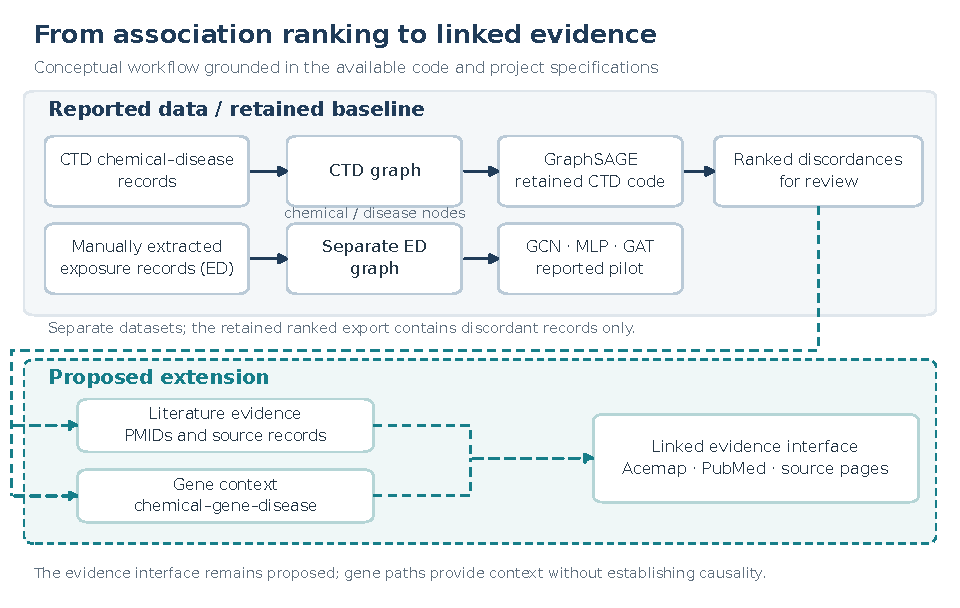
\includegraphics[width=\linewidth]{workflow.pdf}
\caption{Organization of association modeling and evidence review. The graph baseline, retrospective screens and interface design are separate components. The indicated extension adds broader chemical coverage, explicit gene relations and resolved literature links; it does not imply that these features were jointly evaluated in a deployed system.}
\label{fig:workflow}
\end{figure}

\section{Results}
\subsection{The exposure-data pilot does not establish a graph-model advantage}
The reported exposure-data pilot uses a graph with 639 chemical nodes and 94 disease nodes. Table~\ref{tab:pilot} gives the original comparison. The MLP has the highest reported accuracy, recall, F1 and AUROC. Its AUROC exceeds that of GAT by 0.0010 and that of GCN by 0.0138. Without repeated runs or paired prediction records, the small difference between MLP and GAT cannot be interpreted as statistically resolved. The result supports retaining a non-graph baseline in future experiments.

\begin{table}[htbp]
\centering
\caption{Preliminary reported performance on the environmental exposure collection. Recall and F1 averaging conventions were not retained with the source table; repeated-run uncertainty and the exact split membership are unavailable. These values were transcribed, not reproduced by retraining.}
\label{tab:pilot}
\begin{tabular}{lrrrr}
\toprule
Method & Accuracy & Recall & F1 & AUROC \\
\midrule
GCN & 0.8342 & 0.8517 & 0.8430 & 0.9254 \\
MLP & 0.8542 & 0.8631 & 0.8587 & 0.9392 \\
GAT & 0.8474 & 0.8473 & 0.8474 & 0.9382 \\
\bottomrule
\end{tabular}
\end{table}

Other project summaries contain binary and multiclass CTD metrics, but their averaging conventions and dataset correspondence cannot be established. They are not pooled with the exposure-data pilot. In particular, no complete GraphSAGE test prediction file or numerical training log supports a GraphSAGE AUROC comparison here.

\subsection{The retained ranking requires class-aware interpretation}
The larger prediction CSV contains 62,042 records, 16,171 distinct chemical names and 6,193 distinct disease names. There are 61,973 distinct name pairs and 69 exact duplicate rows beyond their first occurrence. Scores range from 0.5000077 to 0.9964914, with a median of 0.7536072. The first 1,000 records contain 805 chemical names, 739 disease names and 998 distinct name pairs (Table~\ref{tab:export}). These counts were calculated directly from the retained file.

\begin{table}[htbp]
\centering\small
\caption{Direct descriptive analysis of the confidence-ranked misclassification export. Distinct names are not equivalent to resolved chemical or disease identifiers.}
\label{tab:export}
\begin{tabular}{lrr}
\toprule
Quantity & Entire export & First 1,000 records \\
\midrule
Records & 62,042 & 1,000 \\
Distinct chemical names & 16,171 & 805 \\
Distinct disease names & 6,193 & 739 \\
Distinct name pairs & 61,973 & 998 \\
Minimum score & 0.5000077 & 0.9793844 \\
Maximum score & 0.9964914 & 0.9964914 \\
\bottomrule
\end{tabular}
\end{table}

The separate ten-record file has scores above 0.9999, all higher than the maximum in the larger export. Its chemical--disease name pairs do not overlap those in the larger file. The two artifacts therefore cannot be interpreted as one internally consistent ranked export. We retain their distinction and do not use the smaller file to supplement the larger ranking.

Most importantly, the export criterion and score definition do not identify a candidate-discovery set. Because both directions of error can be included and class labels are absent, a high-confidence discordance does not demonstrate a predicted positive association. A discovery-oriented export would instead select pairs outside a frozen known-edge set and rank their positive-class scores, while retaining identifiers, labels, run identity and evidence provenance.

\subsection{Reported literature yield is higher in the leading rank window}
The expanded literature screen reports yields of 30.4\%, 19.3\%, 15.8\%, 15.5\%, 14.5\%, 14.4\% and 17.8\% across the seven 1,000-record windows (Figure~\ref{fig:rank}). Yield decreases across the first six windows, then increases in the last window. Within the leading 1,000 records, the ten 100-record bins range from 21\% to 38\% and are not monotonic. The pattern suggests that the highest-ranked sample contains more retrievable literature than much of the remainder, but it does not establish a calibrated relationship between a model score and biological truth.

\begin{figure}[htbp]
\centering
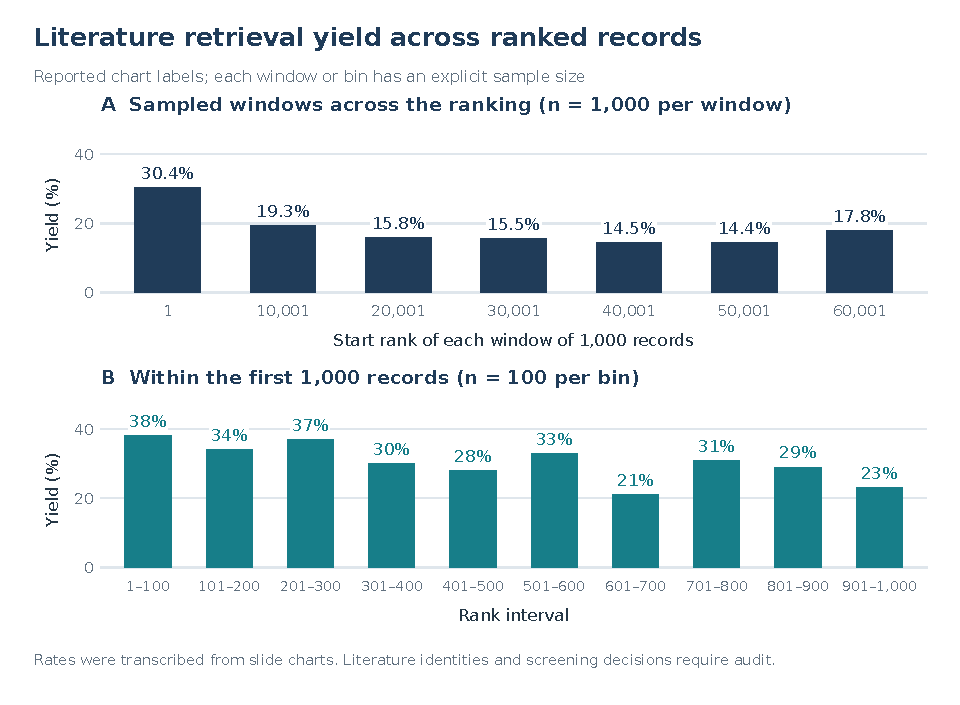
\includegraphics[width=\linewidth]{literature_rank.pdf}
\caption{Retrospective literature-retrieval summaries reconstructed from reported chart labels. Top: seven 1,000-record windows, spaced 10,000 ranks apart. Bottom: ten consecutive 100-record bins within the first window. The horizontal coordinate is rank, not an assumed mean association probability. The summaries lack per-record adjudication and a verified mapping to a versioned positive-prediction set.}
\label{fig:rank}
\end{figure}

The leading window contains 304 reported literature-supported records, compared with 72 among 1,000 randomly paired names. The absolute difference is 23.2 percentage points and the descriptive yield ratio is $304/72=4.22$ (Figure~\ref{fig:support}). This random sample is a vocabulary-based comparator. It is not matched on node degree, literature availability or chemical category, and it is not a temporal validation set. Consequently, the ratio cannot be interpreted as a fourfold increase in the probability of discovering a new true relationship.

\subsection{Shared-gene paths are incomplete and not enriched against the recorded comparator}
In the gene screen, 639 of the first 1,000 ranked records were mappable on both sides. Of those, 128 had at least one shared gene, giving a conditional rate of $128/639=20.0\%$. The overall rate is $128/1{,}000=12.8\%$, with 361 records outside the mappable subset. The retained permutation chart reports an average overall rate of 18.7\%, 5.9 percentage points above the observed rate (Figure~\ref{fig:support}). The screen therefore does not provide descriptive evidence of shared-gene enrichment for the selected ranking.

\begin{figure}[htbp]
\centering
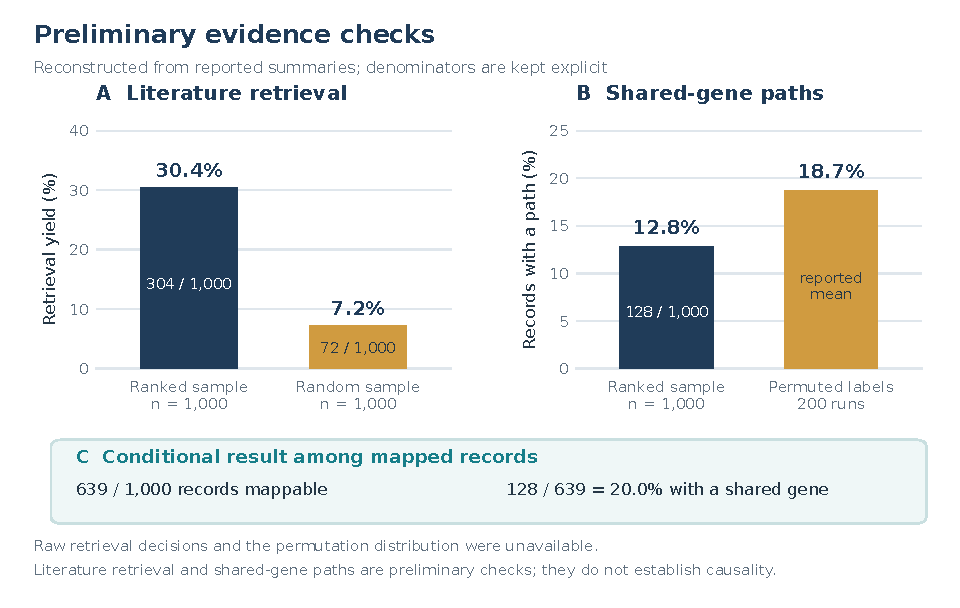
\includegraphics[width=\linewidth]{evidence_support.pdf}
\caption{Two distinct evidence outcomes. Literature yields are aggregate reported results for ranked and random samples. Gene-path coverage uses an all-record denominator of 1,000 for comparison with the disease-label permutation mean; 20.0\% instead conditions on 639 mappable records. The permutation distribution and per-record literature judgments were not retained, so no uncertainty bars or significance claims are added.}
\label{fig:support}
\end{figure}

Reported path examples include vacuolin-1--PIKFYVE--fleck corneal dystrophy, uranium compounds--SRY--46,XY sex reversal 1, and strontium--CASR--familial hypocalciuric hypercalcemia type 1. These examples illustrate connectivity in the selected gene sets. They do not determine the effect of exposure, the direction of regulation or a causal disease mechanism. Since both prediction data and gene context originate from CTD-related resources, path overlap also cannot be assumed to constitute independent validation.

\subsection{Case references illustrate why relation typing is necessary}
The inspected publications support different interpretations (Table~\ref{tab:cases}). Sulfamethoxazole and acute generalized exanthematous pustulosis appear in a case report with a positive lymphocyte transformation test \citep{anliker}. The lithium example concerns hyperosmolar nonketotic coma with a hypothesized indirect pathway through suspected lithium-associated nephrogenic diabetes insipidus \citep{azam}. The octreotide paper reports treatment of pancreatic pseudocysts \citep{gullo}. Thus, finding literature for a chemical--disease pair can recover an adverse reaction, an indirect clinical pathway or a therapeutic effect.

\begin{table}[htbp]
\centering\small
\caption{Illustrative literature-retrieval cases. These are previously published reports recovered for interpretation, not prospectively validated discoveries. PubMed identifiers link to the corresponding records.}
\label{tab:cases}
\begin{tabular}{p{0.20\linewidth}p{0.26\linewidth}p{0.28\linewidth}p{0.13\linewidth}}
\toprule
Chemical & Disease or condition & Supported interpretation & PMID \\
\midrule
Sulfamethoxazole & Acute generalized exanthematous pustulosis & Drug-associated adverse reaction; case-level evidence & \href{https://pubmed.ncbi.nlm.nih.gov/12861854/}{12861854} \\
Lithium & Hyperosmolar nonketotic coma & Hypothesized indirect pathway through nephrogenic diabetes insipidus & \href{https://pubmed.ncbi.nlm.nih.gov/9538487/}{9538487} \\
Octreotide & Pancreatic pseudocysts & Therapeutic use in a clinical report & \href{https://pubmed.ncbi.nlm.nih.gov/1678802/}{1678802} \\
\bottomrule
\end{tabular}
\end{table}

These cases justify keeping article-level evidence separate from a binary ``supported'' badge. A useful evidence view must state what the article actually reports, preserve its study setting, and distinguish direct support from a related mechanism or broader discussion. None of these three reports establishes environmental population risk for the corresponding chemical.

\section{Discussion}
\subsection{Implications for association discovery}
The reported literature yields provide a reason to investigate score-guided review further, but the most defensible current outcome is the organization of potentially relevant literature leads. The class-ambiguous export prevents interpretation of its leading records as novel positive predictions. Even after correcting the export, literature-based assessment would need to distinguish rediscovery from evidence published after the graph was frozen. Publications already underlying CTD cannot serve simultaneously as training evidence and independent confirmation of a prediction derived from that evidence.

The exposure-data comparison also places a useful constraint on model claims. The MLP is numerically competitive with or better than the two reported graph models. This may reflect the dataset, split, sampling scheme or the usefulness of learned entity identities; the current evidence cannot separate those explanations. A graph model should be justified by evaluation on matched splits and appropriate simple baselines, not by the presence of graph-structured data alone.

Gene overlap provides a second caution. Conditioning on mappable records changes the reported rate from 12.8\% to 20.0\%, but it does not improve the comparison against a null that uses all 1,000 records. The observed rate remains below the recorded permutation mean. This result argues for investigating mapping quality, chemical and disease coverage, and gene-degree effects before treating shared paths as corroboration. A gene can participate in many recorded relationships without mediating the specific chemical--disease association being reviewed.

\subsection{A broader chemical resource with traceable evidence}
The system should represent ``chemical'' as the general entity class and retain pollutant, pharmaceutical, endogenous compound, mixture and other categories as explicit annotations where justified. A CAS number or a database name should not silently collapse a mixture, a chemical class and a single molecular structure. Source identifiers and mapping decisions should be preserved alongside display names. Extending the resource in this way increases scope while keeping environmental exposure questions distinguishable from drug-repurposing questions.

Closer Acemap integration is most useful at the evidence item rather than the search-page level. A candidate relationship should expose its PMID, DOI, resolved Acemap article record and relevant source webpage. A failed or ambiguous resolution should remain visible instead of silently linking to a similarly titled paper. The planned evidence record would also carry the quoted supporting passage, relation type, study design, organism, dose or concentration, timing and adjudication status. These fields would allow users to assess whether the link supports the specific claim under consideration.

Gene nodes should be added with typed relations such as chemical--gene interaction and gene--disease association. CTD already supports integrated mechanistic exploration, including connections among chemicals, genes, phenotypes and diseases \citep{ctd2023}; the intended contribution here is their traceable use within this workflow. Edge direction, biological effect and evidence source need to accompany the topology. For prediction, a heterogeneous graph may integrate these relations; for explanation, the interface should display the actual supporting path and its publications. An explanation path need not be a feature used by the predictor, and the interface should state whether it was part of the training graph, added after prediction or obtained from an independent source. The present overlap screen is a starting point for such a view, not a validated mechanism model.

\subsection{Evaluation needed to distinguish retrieval, prediction and validation}
A confirmatory evaluation should begin with an immutable, dated graph snapshot and unique pair-level splits. All occurrences of a held-out pair must be excluded from training labels and message-passing edges. In a heterogeneous model, derived edges that encode a held-out target require separate leakage checks. Random transductive evaluation should be complemented by chemical-disjoint, disease-disjoint and temporal tests. The ID-embedding baseline cannot by itself establish performance for unseen entities; that setting requires explicit handling of new nodes and their features.

The comparator set should include degree-based scoring, an embedding MLP and matched graph models, with the same data, sampling, tuning budget and candidate universe. Average precision, precision at a fixed review budget and calibration are useful alongside AUROC because real candidate spaces are not balanced collections of known positives and sampled unknowns. Repeated seeds and paired uncertainty estimates are needed before claiming model differences.

Literature assessment should predefine the query procedure and evidence categories, conceal model scores from reviewers where feasible, and retain pair-level judgments. A time cutoff should separate prior literature from genuinely subsequent evidence. Random and degree-matched controls address different questions and should both be named accurately. For gene context, mapping coverage and path rate should be reported together, and null comparisons should account for gene-degree and source overlap. These procedures are a prospective validation design, not experiments completed in the present study; a concrete specification is provided in Supplementary Information, Section S6.

\subsection{Limitations}
The study relies partly on aggregate experimental summaries. Missing source snapshots, split manifests and complete labeled predictions prevent reproduction of the historical model metrics and literature yields. The retained training sources contain incompatible entry points and do not constitute a verified execution environment for every reported baseline. No repeated-run variability, deployment benchmark, controlled user study or independent biological experiment is available.

The CTD-based binary task collapses evidence with different meanings, and the negative class comprises unobserved pairs rather than established non-associations. Record-level splitting and repeated samples may make evaluation optimistic. Literature retrieval can favor well-studied entities, can return therapeutic evidence for an adverse-association question, and can reuse the database's own supporting publications. Name-based gene mapping can miss valid identifiers or merge incompatible names; gene-set intersection discards dose, direction and context. These limitations constrain the results to exploratory association review.

\section{Conclusions}
The existing chemical--disease work supports an exploratory workflow combining graph-based scoring with accessible literature and gene-context views. The reported leading-window literature yield is higher than that of random name pairs, while the available gene screen shows no enrichment relative to its recorded permutation mean. Prediction-export semantics and relation typing are decisive for interpretation. Broader chemical coverage, resolved Acemap links and explicit gene relations provide a coherent direction for system development, with claims of discovery requiring reproducible positive predictions and independent supporting evidence.

\section*{Abbreviations}
AUROC, area under the receiver operating characteristic curve; CAS, Chemical Abstracts Service; CTD, Comparative Toxicogenomics Database; GAT, graph attention network; GCN, graph convolutional network; MLP, multilayer perceptron; PMID, PubMed identifier.

\section*{Declarations}
\subsection*{Availability of data and materials}
CTD is available at \url{https://ctdbase.org/}, subject to its source terms. This manuscript is accompanied by supplementary methods, chart-level data provenance and scripts for the descriptive analyses and figures. The original study snapshots, full labeled model outputs and per-record literature judgments are not available in the analyzed research materials; consequently, this package does not reproduce the original training or retrieval experiments. Public deposition details are left blank below pending an author-approved release.
\blankfield{Data/code repository:}
\subsection*{Ethics approval and consent to participate}
\rule{0.95\linewidth}{0.3pt}
\subsection*{Consent for publication}
\rule{0.95\linewidth}{0.3pt}
\subsection*{Competing interests}
\rule{0.95\linewidth}{0.3pt}
\subsection*{Funding}
\rule{0.95\linewidth}{0.3pt}
\subsection*{Authors' contributions}
\rule{0.95\linewidth}{0.3pt}
\subsection*{Acknowledgements}
\rule{0.95\linewidth}{0.3pt}

\begingroup
\small
\setlength{\bibsep}{3pt}
\begin{thebibliography}{99}
\bibitem{ctd2025} Davis AP, Wiegers TC, Sciaky D, et al. Comparative Toxicogenomics Database's 20th anniversary: update 2025. \textit{Nucleic Acids Res.} 2025;53(D1):D1328--D1334. \href{https://doi.org/10.1093/nar/gkae883}{doi:10.1093/nar/gkae883}.
\bibitem{gcn} Kipf TN, Welling M. Semi-Supervised Classification with Graph Convolutional Networks. \textit{International Conference on Learning Representations}. 2017. \url{https://arxiv.org/abs/1609.02907}.
\bibitem{gat} Veli\v{c}kovi\'{c} P, Cucurull G, Casanova A, Romero A, Li\`o P, Bengio Y. Graph Attention Networks. \textit{International Conference on Learning Representations}. 2018. \url{https://arxiv.org/abs/1710.10903}.
\bibitem{graphsage} Hamilton WL, Ying R, Leskovec J. Inductive Representation Learning on Large Graphs. \textit{Advances in Neural Information Processing Systems}. 2017;30. \url{https://arxiv.org/abs/1706.02216}.
\bibitem{lagcn} Yu Z, Huang F, Zhao X, Xiao W, Zhang W. Predicting drug--disease associations through layer attention graph convolutional network. \textit{Brief Bioinform.} 2021;22(4):bbaa243. \href{https://doi.org/10.1093/bib/bbaa243}{doi:10.1093/bib/bbaa243}.
\bibitem{mrdda} Chen C, Zhou Y, Li Y, Xu J, Li D, Wang L. MRDDA: a multi-relational graph neural network for drug--disease association prediction. \textit{J Transl Med.} 2025;23:753. \href{https://doi.org/10.1186/s12967-025-06783-x}{doi:10.1186/s12967-025-06783-x}.
\bibitem{sider} Kuhn M, Letunic I, Jensen LJ, Bork P. The SIDER database of drugs and side effects. \textit{Nucleic Acids Res.} 2016;44(D1):D1075--D1079. \href{https://doi.org/10.1093/nar/gkv1075}{doi:10.1093/nar/gkv1075}.
\bibitem{lightgcn} He X, Deng K, Wang X, Li Y, Zhang Y, Wang M. LightGCN: Simplifying and Powering Graph Convolution Network for Recommendation. \textit{Proceedings of SIGIR}. 2020:639--648. \href{https://doi.org/10.1145/3397271.3401063}{doi:10.1145/3397271.3401063}.
\bibitem{node2vec} Grover A, Leskovec J. node2vec: Scalable Feature Learning for Networks. \textit{Proceedings of KDD}. 2016:855--864. \href{https://doi.org/10.1145/2939672.2939754}{doi:10.1145/2939672.2939754}.
\bibitem{acemap} Tan Z, Liu C, Mao Y, Guo Y, Shen J, Wang X. AceMap: A Novel Approach towards Displaying Relationship among Academic Literatures. \textit{Proceedings of the 25th International Conference Companion on World Wide Web}. 2016:437--442. \href{https://doi.org/10.1145/2872518.2890514}{doi:10.1145/2872518.2890514}.
\bibitem{anliker} Anliker MD, W\"uthrich B. Acute generalized exanthematous pustulosis due to sulfamethoxazol with positive lymphocyte transformation test (LTT). \textit{J Investig Allergol Clin Immunol.} 2003;13(1):66--68. \url{https://pubmed.ncbi.nlm.nih.gov/12861854/}.
\bibitem{azam} Azam H, Newton RW, Morris AD, Thompson CJ. Hyperosmolar nonketotic coma precipitated by lithium-induced nephrogenic diabetes insipidus. \textit{Postgrad Med J.} 1998;74(867):39--41. \href{https://doi.org/10.1136/pgmj.74.867.39}{doi:10.1136/pgmj.74.867.39}.
\bibitem{gullo} Gullo L, Barbara L. Treatment of pancreatic pseudocysts with octreotide. \textit{Lancet}. 1991;338(8766):540--541. \href{https://doi.org/10.1016/0140-6736(91)91102-z}{doi:10.1016/0140-6736(91)91102-z}.
\bibitem{ctd2023} Davis AP, Wiegers TC, Johnson RJ, Sciaky D, Wiegers J, Mattingly CJ. Comparative Toxicogenomics Database (CTD): update 2023. \textit{Nucleic Acids Res.} 2023;51(D1):D1257--D1262. \href{https://doi.org/10.1093/nar/gkac833}{doi:10.1093/nar/gkac833}.
\end{thebibliography}

\endgroup

\end{document}
